%%%% Better Poster latex template example v1.0 (2019/04/04)
%%%% GNU General Public License v3.0
%%%% Rafael Bailo
%%%% https://github.com/rafaelbailo/betterposter-latex-template
%%%%
%%%% Original design from Mike Morrison
%%%% https://twitter.com/mikemorrison

\documentclass[a2paper,fleqn]{betterposter}

%%%% Uncomment the following commands to customise the format

% Setting the width of columns
\setlength{\leftbarwidth}{0.25\paperwidth}
\setlength{\rightbarwidth}{0.25\paperwidth}

%% Setting the column margins
% Horizontal margin
%\setlength{\columnmarginvertical}{0.05\paperheight}
% Vertical margin
%\setlength{\columnmarginhorizontal}{0.05\paperheight}
% Horizontal margin for the main column
%\setlength{\maincolumnmarginvertical}{0.15\paperheight}
% Vertical margin for the main column
%\setlength{\maincolumnmarginhorizontal}{0.15\paperheight}

%% Changing font sizes
% Text font
%\renewcommand{\fontsizestandard}{\fontsize{28}{35} \selectfont}
% Main column font
%\renewcommand{\fontsizemain}{\fontsize{28}{35} \selectfont}
% Title font
\renewcommand{\fontsizetitle}{\fontsize{28}{35} \selectfont}
% Author font
%\renewcommand{\fontsizeauthor}{\fontsize{28}{35} \selectfont}
% Section font
%\renewcommand{\fontsizesection}{\fontsize{28}{35} \selectfont}

%% Changing font sizes for a specific text segment
% Place the text inside brackets:
% {\fontsize{28}{35} \selectfont Your text goes here}

%% Changing colours
% Background of side columns
%\renewcommand{\columnbackgroundcolor}{black}
% Font of side columns
%\renewcommand{\columnfontcolor}{gray}
% Background of main column
%\renewcommand{\maincolumnbackgroundcolor}{empirical}
%\renewcommand{\maincolumnbackgroundcolor}{theory}
%\renewcommand{\maincolumnbackgroundcolor}{methods}
%\renewcommand{\maincolumnbackgroundcolor}{intervention}
% Font of main column
%\renewcommand{\maincolumnfontcolor}{gray}

\begin{document}
\betterposter{
%%%%%%%% MAIN COLUMN

\maincolumn{
%%%% Main space
Keep your GraphQL API \textbf{secure}, while still have a strong
\textbf{documentation}, \textbf{without} Introspection.
}{
%%%% Bottom space

%% QR code
\qrcode{img/frame}{img/smartphoneWhite}{
\textbf{Take a picture} to
\\download the full paper
}
% Smartphone icon
% Author: Freepik
% Retrieved from: https://www.flaticon.com/free-icon/smartphone_65680

%% Compact QR code (comment the previous command and uncomment this one to switch)
%\compactqrcode{img/qrcode}{
%\textbf{Take a picture} to
%\\download the full paper
%}

}

}{
%%%%%%%% LEFT COLUMN

\title{Markdown Generation from a GraphQL Schema}
\author{Alessandro Buonerba}
\institution{University of Greenwich}

\section{Abstract}
Since GraphQL was publicly released in 2015, many developers adopted it to
create new public faced APIs, but these are often poorly documented. Writing
well-structured documentation requires time and manual work, and the tooling
currently available at the time of this paper would require technologies and
frameworks lock-in. This project aims to generate markdown files that can then
be parsed in any framework of choice. Since the output will be in Markdown, the
user can then use his parser to manipulate the documents and produce static
files for their frontend.

\section{Introduction}
Documentation is a crucial aspect of the development of software. It is so
important that every developer building a GraphQL API should be aware of it an
keeping their Schemas documented to enable and facilitate consumers to
understand how to use the API. A very a good way to document such APIs is not
to be locked in with any vendor-specific that generates documentation on the fly
given a specific schema but building static documentation that automatically
updates on the fly when a change is made to it. The following literature review
will point the differences between different APIs, analyse and critically
evaluate the options developers have to reach the same goal and why the software
implementation of the tool used in the project gives the producers better
results, freedom and save them money. Security implications are also another
important aspect of the lifecycle and this paper will dive into analysis and
confrontation to understand this.

}{
%%%%%%%% RIGHT COLUMN
\section{Methods}
\begin{itemize}
\item Construct a GraphQL Schema
\item Generate an AST object
\item Manipulate the object
\item Generate a Markdown file
\item Recursively for each field and type
\end{itemize}

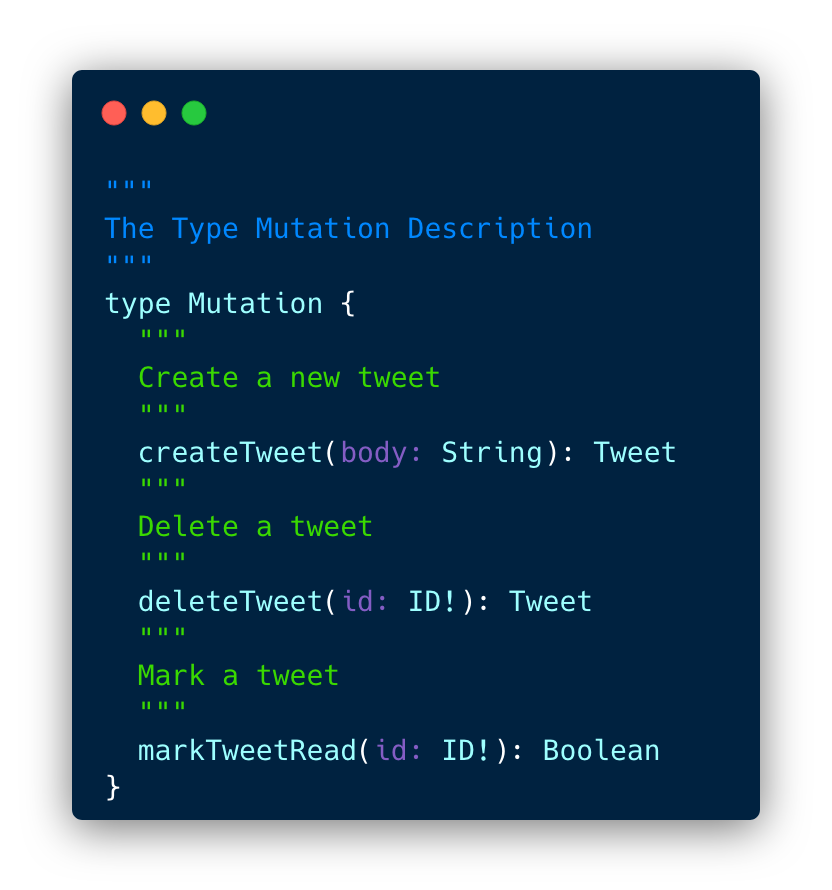
\includegraphics[width=\textwidth]{img/graphql}
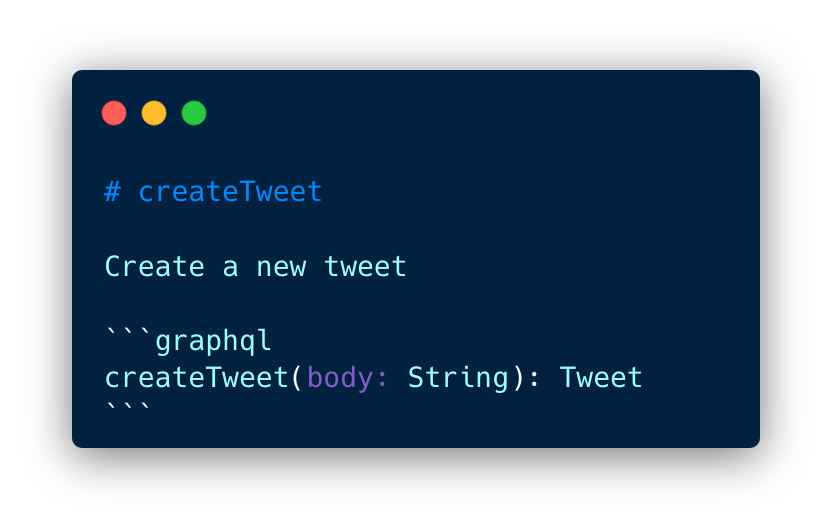
\includegraphics[width=\textwidth]{img/markdown}

\section{Output}
\\
\fbox{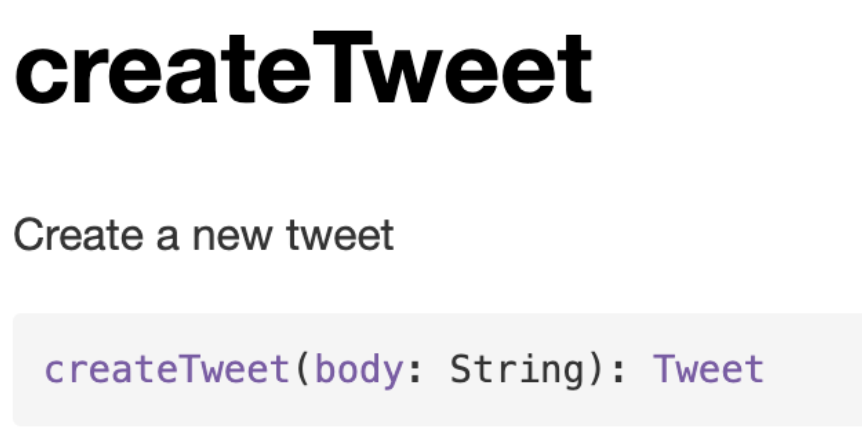
\includegraphics[width=\textwidth]{img/output}}
}
\end{document}
